% --------------------------------------
%       PLEASE SEE README.MD
% --------------------------------------

\documentclass[
    letterpaper,
    10pt,
    unnumberedsections,
    twoside
]{LTJournalArticle}

\runninghead{Biomimetic Hydrogel-Scaffold for Tendon and Ligament Repair}
\footertext{}

\usepackage{lipsum} % Lorem ipsum text for formatting
\usepackage{chemfig}
\usepackage{dblfloatfix}

\addbibresource{references_lucas.bib}
\addbibresource{references_edison.bib}
\addbibresource{references_luke.bib}
\addbibresource{references_matt.bib}

\title{Biomimetic Hydrogel-Scaffold for Tendon and Ligament Repair}
\author{Lucas Chan, Luke Gailloux, Matt Levasseur, Edison Luke}

\renewcommand{\maketitlehookd}{%
    \begin{abstract}
        \noindent \lipsum[1]
    \end{abstract}
}

\setlength{\parskip}{0pt plus 1pt}

\begin{document}
    \maketitle 

    \section{Introduction}

    Sample introduction for formatting testing.

\lipsum[1]

    \section{Hydrogel Structure and Composition}

    Hydrogels are 3D crosslinked polymer structures containing hydrohpilic functional groups, allowing them to absorb large quantities of water. Because of this, they are flexible and soft, and resemble many natural tissues \autocite{hoHydrogelsPropertiesApplications2022}.
Recent advances in hydrogel technology have led to the development of implantable and injectable hydrogels with potential applications in drug delivery. By adjusting polymer composition, key properties such as swelling-deswelling rate, stiffness, and degradability can be fine-tuned to meet specific use case requirements. As biomedical applications of hydrogels continue to expand, their use in tendon and ligament repair presents a promising opportunity.

Hydrogel cross-linked chains can be formed using natural, synthetic, or semi-synthetic polymers. Natural polymers such as cellulose, chitosan, and collagen are inherently biocompatible and bioactive, but come at the cost of weak stability and poor mechanical strength. Being derived from natural sources, these hydrogels are generally safe to use in clinical applications, but have shown to be allergens in rare cases \autocite{hoHydrogelsPropertiesApplications2022}.

On the other hand, synthetic hydrogels are made of man-made polymers like polyvinyl alcohol (PVA), polyethylene glycol (PVG), or polyacrylamide (PAAM). Few of these synthetic materials have been shown to be biocompatible, but they offer superior mechanical strength and stability \autocite{hoHydrogelsPropertiesApplications2022}.

To achieve both the biocompatibility offered by natural hydrogels and the strength and mechanical properties offered by their synthetic counterparts, a common approach is to develop a hybrid, or semi-synthetic hydrogel chain. Hybrid hydrogels can either be made by chemically modifying natural polymers or by blending natural and synthetic components.

    \section{Self-Healing ``Smart'' Hydrogels}

    When subjected to physical or chemical stimuli, ``smart'' hydrogels have the ability to dynamically modify their physical properties, such as mechanical strength and swellability \autocite{hoHydrogelsPropertiesApplications2022}.
Self-healing hydrogels are a subset of smart hydrogels. These hydrogels are made of dynamic cross-linkages that can spontaneously re-form after having sustained mechanical damage. Self-healing properties allow the hydrogel to have superior mechanical toughness and a longer life span \autocite{deviv.k.SelfHealingHydrogelsPreparation2021}.

Self-healing hydrogels are unique in that the polymer chains are bound together by dynamic cross-linkages that can spontaneously self-repair. These cross-linkages can be the result of covalent or non-covalent interactions.
Covalent cross-linkages include imine and disulfide bonds. They are higher in energy and are therefore more difficult to break. Because of this, they are generally more stable and have superior mechanical strength.
Reversible non-covalent dynamic linkages arise from interactions such as hydrogen bonding, ionic interactions, and hydrophobic effects. These bonds are easily broken and reconstructed, which leads to a more flexible but mechanically weaker hydrogel \autocite{deviv.k.SelfHealingHydrogelsPreparation2021}.

\subsection{Self-Healing by Imine Bonds}

Imine bonds for self-healing hydrogels show promise in biomedical applications, especially in wound healing and in tissue engineering. Imines are chemical compounds containing a carbon atom doubly-bonded to a nitrogen. They are stabilised when the nitrogen atom contains an aromatic ring as a substituent, in which case it is known as a Schiff base \autocite{moldoveanuChapter8Pyrolysis2019}.
The C=N imine bond is formed when an aldehyde reacts with an amine, forming the Schiff base. This reaction is reversible, meaning that the imine bond can break and reform spontaneously given the appropriate conditions.

\begin{figure}[ht]
    \setchemfig{atom sep=2em}
    \centering
    \chemfig{
        *6((-R_1)=-=(-=[::-60]N-R_2)-=-)
    }
    \caption{Bond-line illustration of a Schiff base}
    \label{fig:schiff_base}
\end{figure}

    \subsection{Janus Interfaces for Optimal Hydrogel Performance}
Hydrogels often integrate janus surfaces to exhibit a boundary-defined contrast in material properties. This boundary can be delimited microscopically or macroscopically and may be either pattern-based or cross-sectional (the material properties will change at the opposing faces of a cross-sectional plane). The Janus surface is a refinement of the Janus bead, developed in 1989, which consists of an amphiphilic glass bead with a cross-sectional wettability contrast \autocite{janus_interface}. The integration of varying wettabilities in a single material is biomimetic: it is inspired by both the carapace of the desert beetle Stenocara sp. and its unique water retrieval mechanism as well as the surface of the lotus leaf and its contrasting wettabilities at the air and water interfaces \autocite{janus_interface}. Janus interface materials now integrate other boundary-contrasted material properties, such as contrasting chemical composition and mechanics. 

\subsection{Janus Tough Adhesives}
The Janus Tough Adhesive is a hydrogel that incorporates a Janus interface and is optimized for biomedical applications, particularly in tissue regeneration for tendon repair \autocite{jta_poc}. One face of the Janus interface allows for strong adhesion of the hydrogel to wet tissue surfaces and the other is designed to facilitate the gliding of surrounding tissues. The latter property is essential to prevent postoperative tissue adhesion, which is a frequent complication of invasive procedures, often resulting in reoperation. The unique properties of the JTA arise from the mixing of ionically crosslinked alginate -with calcium ions- and covalently crosslinked polyacrylamide \autocite{jta_poc}. Application of a chitosan-containing mixture on one side results in the highly adhesive character at the tendon interface of the hydrogel. JTAs are remarkable as they integrate either adhesive or gliding properties at its interfaces while maintaining uniformly high toughness. 



    \section{Mechanical Properties of Janus Tough Adhesive Hydrogels}

    In addition to biocompatibility, the mechanical properties of a given hydrogel decide whether or not a given hydrogel is functional. In particular, hydrogels must have sufficient toughness and adhesive strength \autocite{Freedman.EnhancedTendonHealing}. In vivo, tendons must withstand a dynamic environment and bear strong forces \autocite{Chen.AdvancesApplicationHydrogel}; thus, a hydrogel must be able to withstand sufficient amounts of force without fracturing – that is, an ideal hydrogel should only deform plastically (Freedman et al.). Furthermore, to promote optimal healing, hydrogels should be placed and remain near the relevant tendon. However, force generated by movement can lead to hydrogel displacement; Hence, adhesion is required to ensure immobility (Freedman et al.). A variety of strategies can be implemented on a biochemical level to greatly increase the toughness and adhesiveness in order to create an adequate hydrogel for tendon repair.

This is still a test
High mechanical toughness of the JTA was achieved using a dual interpenetrating hydrogel network that combines the ability of alginate hydrogels to dissipate energy through dissociation of ionic bonds with a highly elastic covalently cross-linked acrylamide hydrogel that can distribute stresses throughout the network. \cite{FreedmanEnhancedTendonHealing}

The backbone structure of the tough SL was polyacrylic acid (PAA) networks, with long-chain glycidyl methacrylate-modified chondroitin sulfate (CSMA) as the cross-linking agent and encapsulated chondroitin sulfate (CS), which endowed the JHA with strong mechanical properties for effectively dissipating energy under deformation \cite{JuSurfaceEnzymePolymerization}

The interlocking structure and continuous features of the JHA were also confirmed from the Raman mapping image in Fig. 2i. This interlocked structure firmly bonded the two layers, and the RL could effectively transfer the strain to the SL through the interlocking structure, avoiding fracture and delamination, thereby achieving stable and robust adhesion to biological tissues. \cite{JuSurfaceEnzymePolymerization}



    \section{Targeted Drug Delivery}

    \subsection{Standard of Care for Drug-Based Therapies}
Hydrogel-based therapies for connective tissue injuries enable improved mechanisms of drug delivery. Novel mechanisms of drug delivery seek to address many of the issues plaguing the effective treatment of disease with drugs. For one, the modest successes of many drug delivery mechanisms are diminished by the drug's bioavailability via its route of administration \autocite{nsaids}. Furthermore, traditional routes of drug administration often require frequent intervals of high drug dosages to induce noticeable effects. These drug administration modalities often diminish the drug-s overall efficacy by reducing patient compliance and increasing overall toxicity to the body \autocite{nsaids}. Drug performance can be improved via localized sustained release, i.e., subjecting the diseased region to uniform and lower drug concentrations locally throughout the course of treatment.

\subsection{Optimization of Hydrogel Composition for Sustained Drug Release}
The tunable nature of the hydrogel makes it a promising candidate to actuate localized and sustained drug release. Hydrogels are hierarchical in nature: macroscopic properties define the route of administration, while the microscopic scale governs convective drug transport and other physical interactions \autocite{mooney_drug}. The mesh scale -several hundred nanometers- governs diffusion of drugs within the polymer network and the molecular scale defines binding interactions between the drugs and the polymers. Hydrogel features at some given length scale can be modified while preserving the hydrogel's general character, i.e., the hydrogel can be modified to optimally suit a medication regimen while retaining its macroscopic mechanical and physical properties \autocite{mooney_drug}.  Relatedly, the high water content within hydrogels entails minimal denaturation of the drugs that are stored within the mesh space. Likewise, the extremely small mesh size resulting from polymer interactions prevents the inward diffusion of enzymes into the matrix and precludes premature degradation of the drugs. 

\subsection{JTAs for Sustained Drug Release}
The mechanical and physical properties of the JTA make it an ideal candidate for the improvement of current drug depot mechanisms. While most depots cannot adhere to the targeted tissue, the adhesive nature of the chitosan coating on the JTA restrains movement and prevents migration on the tissue. Likewise, the hydrogel resists mechanical disintegration due to its toughness and can thus avert burst release of the drug. The miniscule mesh size of the JTA impairs diffusion-based drug release, resulting in the almost exclusive release of a drug by dissolution, which suggests an effective method for delivering hydrophobic drugs to the diseased tissue \autocite{jta_poc}. Using triamcinolone acetonide as a model drug, a corticosteroid, it was found that the hydrogel could sustain stable drug release over a 10-day interval under perfect sink conditions. Additionally, while current standard of care suffers from poor loading capacities (0.01-1mg/ml), the JTA can support loading of drug concentrations up to 5000 times this amount, emphasizing the benefit of its use for long-term therapeutic goals \autocite{jta_poc}. Targeted drug therapies present a unique opportunity to tailor medication regimens to preserve the beneficial aspects of some drugs while mitigating their undesirable effects at a local scale.

\subsection{JTAs as Vehicles for Stem Cell Therapy}
Stem cell therapy proposes promising solutions to issues plaguing tendon mechanical performance post-injury. Indeed, the hypocellularity of tendon tissues results in extrinsic mechanisms for healing, which generate scar tissue and reduce the structural quality of the tendon. On account of their remarkable compatibility with encapsulated stem cells, hydrogels are proposed as means of delivering stem cells to hypocellular tissues to bolster intrinsic healing processes \autocite{intro}. When implanted at the site of the injured tendon, stem cells are expected to differentiate into the tenogenic lineage and regenerate the damaged tendon with a composition and structure native to this type of tissue. Furthermore, the secretion of paracrine factors by stem cells would enhance cellular proliferation and migration in nearby cells, intensifying intrinsic healing of the tendon. The functional adaptability of hydrogels provides a direct way to encourage proper onsite cell differentiation, as hydrogel topography, mechanics, and chemistry can all be significantly altered to induce tenogenic differentiation of stem cells \autocite{intro}. As research concerning tendon healing is sluggish relative to other musculoskeletal tissues, the time at which stem cell delivery would yield optimal outcomes is yet unresolved. However, hydrogels offer immense variability in terms of time scales of degradation and could accommodate several courses of treatment. 

    \section{Biocompatibility}

    The Janus Tough Adhesive has shown to exhibit high biocompatibility during testing, despite it containing the synthetic polymer polyacrylamide. To evaluate their performance and impact on natural tissues, \citeauthor{freedmanEnhancedTendonHealing2022} (\citeyear{freedmanEnhancedTendonHealing2022}) experimentally tested  injured and healthy rats, and applied the JTA to the patellar tendon.
For three weeks, potential swelling of the tendon and degredation of the gel were assessed by high frequency ultrasound. When a tendon becomes injured, its echogenicity---the amount of sound it reflects---decreases, because its collagen fibres become more disorganised and less densely packed \autocite{hodgsonTendonLigamentImaging2012}.
Researchers also found that injured tendons without application of the JTA had larger cross-section areas, indicating increased swelling as shown in Figure~\ref{fig:JTA_Patellar_cross_section}. A decrease in inflammation in the affected tendon therefore suggests that the JTA was effective and well-tolerated by the body.
\begin{figure*}[ht]
    \centering
    \begin{minipage}[b]{0.45\textwidth}
        \centering
        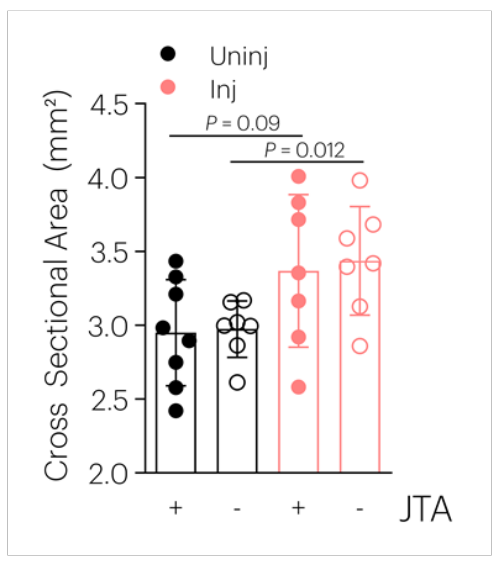
\includegraphics[width=0.6\linewidth]{JTA_cross_section.png}
        \caption{Patellar tendon cross-sectional area (mm\textsuperscript{2}) after 3 weeks of treatment [Adapted from \cite{freedmanEnhancedTendonHealing2022}]}
        \label{fig:JTA_Patellar_cross_section}
    \end{minipage}
    \hfill
    \begin{minipage}[b]{0.45\textwidth}
        \centering
        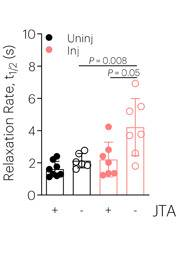
\includegraphics[width=0.6\linewidth]{Figures/JTA_relaxation_patellar.jpeg}
        \caption{Patellar tendon relaxation rate [Adapted from \cite{freedmanEnhancedTendonHealing2022}]}
        \label{fig:JTA_Patellar_relaxation}
    \end{minipage}
\end{figure*}

Furthermore, in the patellar tendon, the JTA was found to have improved tendon relaxation (Figure~\ref{fig:JTA_Patellar_relaxation}), without impacting natural properties such as elastic mechanics, dynamic modulus, or linear modulus.

% Biocompatibility of the JTA was also tested in more complex use cases, such as the rotator cuff and Achilles tendon. 

    \section{Degradation of the Hydrogel Scaffold}

    As the goal of a hydrogel scaffold is to promote natural healing, it must degrade over time to
allow the naturally-formed tissue to take over, yet its lifespan must be long enough to
continuously support the afflicted area throughout the healing process. Tendon and ligament
repair is a lengthy process that can take several months to over a year for full healing \autocite{RN1}. Traditional polymer-based hydrogels degrade too quickly to be effective in long healing
processes. Depending on the specific chemical composition, these hydrogels can degrade
within the body in less than 6 months due to hydrolysis, oxidization, and enzymatic activity.
Therefore, the use of a composite hydrogel becomes absolutely necessary for use in
tendon repair.

Composite hydrogels incorporate blends of natural and synthetic materials and linkage
structures such as double networks and interpenetrating networks. These hydrogels not only
last longer than natural or synthetic polymer-based hydrogels, but are also tunable, as their
lifespan can be modified by adjusting the cross-linking type and density. This allows for
improved customizability while maintaining permeability and resisting premature degradation. In
addition, the hydrogel structure can be engineered to respond to environmental stimuli such as
pH and enzyme presence, allowing them to be dynamic and responsive to the state of the
healing tissue, gradually breaking down in sync with tissue regeneration \autocite{RN3}.

\subsection{Effects of Crosslinking on Hydrogel Degradation
}

As mentioned above, composite hydrogels are highly customizable. Their lifespan may be
customized to better fit the timeline of the specific injury being treated. One such technique is
modifying the crosslinking density between hydrogel layers. A study by \citeauthor{RN4} found that an
increased concentration of glutaraldehyde crosslinking correlates with higher mechanical
strength and lower degradation rates (\citeyear{RN4}). Greater crosslinking forms a denser polymer network,
making the hydrogel more resistant to breakdown from oxidation, hydrolysis, and enzymatic
activity.

\subsection{Degradation of the JTA}

% Figure for Self-Healing,
% need to include here for correct positioning
\begin{figure*}[b]
    \centering 
    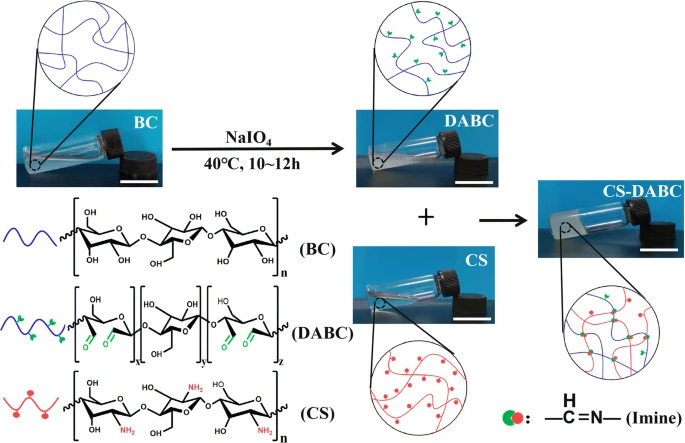
\includegraphics[width=0.7\linewidth]{Figures/CS_DABC_condensation.jpg}
    \caption{Schematic representation of hydrogel synthesis from chitosan and dialdehyde bacterial cellulose \autocite{liAllnaturalInjectableHydrogel2020}}
    \label{fig:CS_DABC_condensation}
\end{figure*}

The JTA combines several natural and synthetic materials, all of which must be safely broken down within the body to serve as an effective treatment. Alginate, a water-soluble polysaccharide which makes up the hydrophilic matrix of the hydrogel, degrades into monosaccharides, primarily guluronic and mannuronic acid units. These are very easily excreted from the body via the renal system. 
Chitosan, a cationic polymer typically used in the bioadhesive layer of the JTA, degrades into glucosamine and N-acetylglucosamine. These monosaccharides are involved in the body's natural metabolic processes, so they are very easily reintegrated into the body's metabolic system following the breakdown of the JTA \autocite{guarinoDegradationPropertiesMetabolic2015}.
Polyacrylamide, a synthetic polymer that makes up the backbone of the double-network structure, breaks down into acrylamide monomers. These synthetic byproducts can either be metabolized by the liver before being excreted via urine, or they can undergo conjugation with glutathione or glutathione-S-transferases, making them non-toxic and water-soluble \autocite{xiongPolyacrylamideDegradationIts2018}.
Schiff base linkages, which provide dynamic crosslinking within the JTA, hydrolyze into aldehydes and amines, which are non-toxic and easily metabolized or excreted \autocite{xuHydrogelsBasedSchiff2019}.

The degradation process roughly follows in the following order, from quickest to slowest degradation: alginate, chitosan, imine bonds, polyacrylamide. This order is very beneficial for the healing process. Alginate and chitosan, being natural components of the hydrogel, degrade quickly within the body, softening it slightly.
This both increases the permeability of the hydrogel, allowing cells and nutrients to enter and exit more efficiently, and encourages integration of the healing tissues with the hydrogel \autocite{RN4}.
Imine bonds provide the self-healing factor of the JTA, allowing it to recover from minor deformations and maintain structural integrity under movement. However, these bonds also degrade over time, after about 1--3 months, allowing more mechanical load to be gradually shifted from the hydrogel onto the recovering tissue \autocite{xuHydrogelsBasedSchiff2019}.
The polyacrylamide backbone, being a synthetic polymer, is the last to degrade within the body. This structure is critical in providing support to the tissue and must degrade approximately synchronously with the recovery time of the injury.

    % Towards a Self-Healing JTA
    % Section header command contained in the subfile
    % for better figure formatting

    \begin{figure*}[hb]
    \centering 
    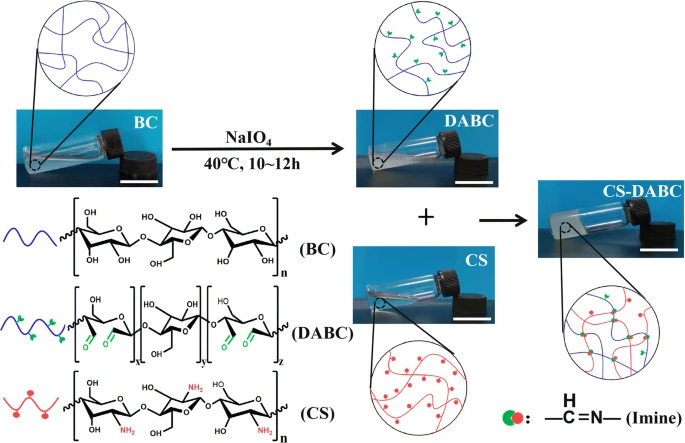
\includegraphics[width=0.7\linewidth]{Figures/CS_DABC_condensation.jpg}
    \caption{Schematic representation of hydrogel synthesis from chitosan and dialdehyde bacterial cellulose \autocite{liAllnaturalInjectableHydrogel2020}}
    \label{fig:CS_DABC_condensation}
\end{figure*}

\section{Towards a Self-Healing JTA}

A recent study by \citeauthor{liAllnaturalInjectableHydrogel2020} found that an all-natural, injectable hydrogel could be synthesized using chitosan and dialdehyde bacterial cellulose (\citeyear{liAllnaturalInjectableHydrogel2020}). This hydrogel uses imine bond dynamic cross-linkages to achieve its self-healing properties, where the Schiff base forms through the reaction of chitosan (as the amine) and bacterial cellulose (as the aldehyde).
The reaction can proceed under mild conditions (room temperature and pH = 7.2), and as it is all-natural, it has shown to be biocompatible. A schematic representation of this condensation reaction is given in Figure~\ref{fig:CS_DABC_condensation}.

Researchers tested the CS-DABC hydrogel's ability to self-repair after sustaining damage, a property that is desired for applications in wound dressings. To do so, round hydrogels were prepared and cut in half. One side was coloured orange, and the two half-discs were placed side-by-side in ambient conditions, as shown in Figure~\ref{fig:CS_DABC_self_healing}.
In just 3 hours, without external intervention, the two halves fused back together and reformed the original shape. They were also able to be picked up by one side, withstanding the force of gravity. Moreover, the gaps between the two hydrogel half-discs were observed under optical microscope.
The boundaries between the two sides were barely visible, demonstrating good self-healing properties from Schiff base reactions.

\begin{figure}[ht]
    \centering 
    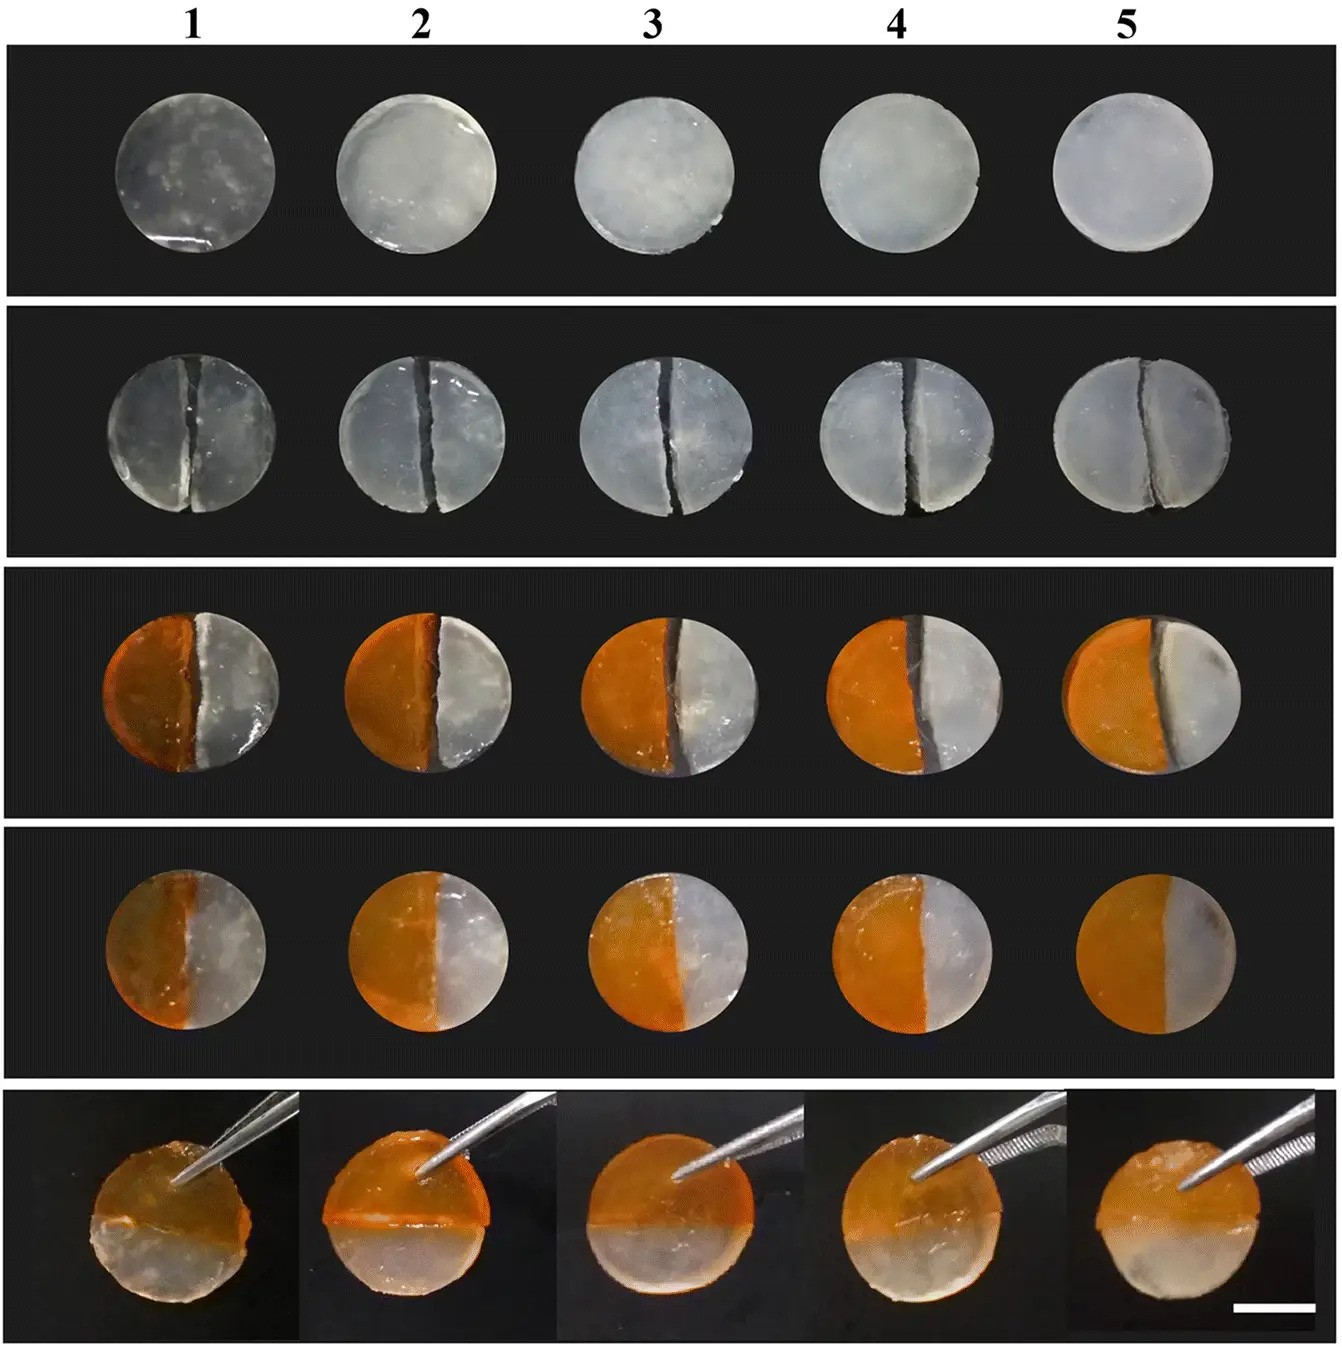
\includegraphics[width=\linewidth]{Figures/CS_DABC_self_healing.jpg}
    \caption{Self-healing properties of CS-DABC hydrogels. Discs were cut, stained, and healed under ambient conditions. [Adapted from \cite{liAllnaturalInjectableHydrogel2020}]}
    \label{fig:CS_DABC_self_healing}
\end{figure}

Additionally, the chitosan dressing exhibits antimicrobial properties, which reduces the risk of cross-contamination and promotes healthy healing of the wound. To evaluate these properties, the hydrogel was tested as an antibiotic against strains of \textit{E. coli} and \textit{S. aureus}.
Far fewer bacterial colonies were observed in the samples treated with CS-DABC compared to the control. As the hydrogel's protonated amino groups bind to the bacterial cell wall, effectively destroying it, bacterial growth is inhibited \autocite{liAllnaturalInjectableHydrogel2020}.

This self-healing hydrogel presents a promising application for tendon repair. Since JTAs already have a chitosan layer, it could be possible to synthesize Schiff bases directly on the existing structure using a similar technique as \citeauthor{liAllnaturalInjectableHydrogel2020}, leading to increased mechanical strength through the integration of self-healing properties.
% This self-healing hydrogel, therefore, has an interesting application for tendon repair. Given that JTAs have a chitosan side, it could be possible to augment their mechanical strength by integrating self-healing properties.

    \onecolumn
    \printbibliography
\end{document}